\documentclass[12pt]{report}

\usepackage[T1]{fontenc}
\usepackage[utf8]{inputenc}
\usepackage{graphicx}
\usepackage{amsmath,amssymb,amsfonts}
\usepackage{txfonts}
\usepackage{pdfpages}
\usepackage{caption}
\usepackage{float}
\usepackage{listings}
\usepackage[polish]{babel}

\renewcommand{\chaptername}{Rozdział}
\renewcommand{\contentsname}{Spis treści}
\renewcommand{\figurename}{Rys.}
\renewcommand{\tablename}{Tab.}
\renewcommand{\listfigurename}{Spis rysunków}
\renewcommand{\listtablename}{Spis tabel}
\renewcommand{\bibname}{Bibliografia}
\renewcommand\lstlistingname{Listing}
\renewcommand\lstlistlistingname{Spis listingów}

\pagestyle{headings}

\setlength{\textwidth}{14cm}
\setlength{\textheight}{20cm}

\newtheorem{definition}{Definicja}
\newtheorem{example}{Przykład}[chapter]
\newtheorem{corollary}{Wniosek}[chapter]

\begin{document}

\lstset{aboveskip=20pt,belowskip=20pt}

\lstdefinestyle{customcmd}{
captionpos=b, 
belowcaptionskip=1\baselineskip,
breaklines=true,
frame=LRTB,
xleftmargin=\parindent,
showstringspaces=false,
basicstyle=\footnotesize\ttfamily
}

\lstdefinestyle{customsql}{
captionpos=b, 
belowcaptionskip=1\baselineskip,
breaklines=true,
frame=LRTB,
xleftmargin=\parindent,
language=SQL,
showstringspaces=false,
basicstyle=\footnotesize\ttfamily,
keywordstyle=\bfseries\color{purple},
identifierstyle=\color{violet}
}

\lstdefinestyle{customc}{
captionpos=b, 
belowcaptionskip=1\baselineskip,
breaklines=true,
frame=LRTB,
xleftmargin=\parindent,
language=C++,
showstringspaces=false,
basicstyle=\footnotesize\ttfamily,
keywordstyle=\bfseries\color{green!40!black},
commentstyle=\itshape\color{purple!40!black},
identifierstyle=\color{blue},
stringstyle=\color{orange},
}

% TODO strona tytułowa i tytuł!
% 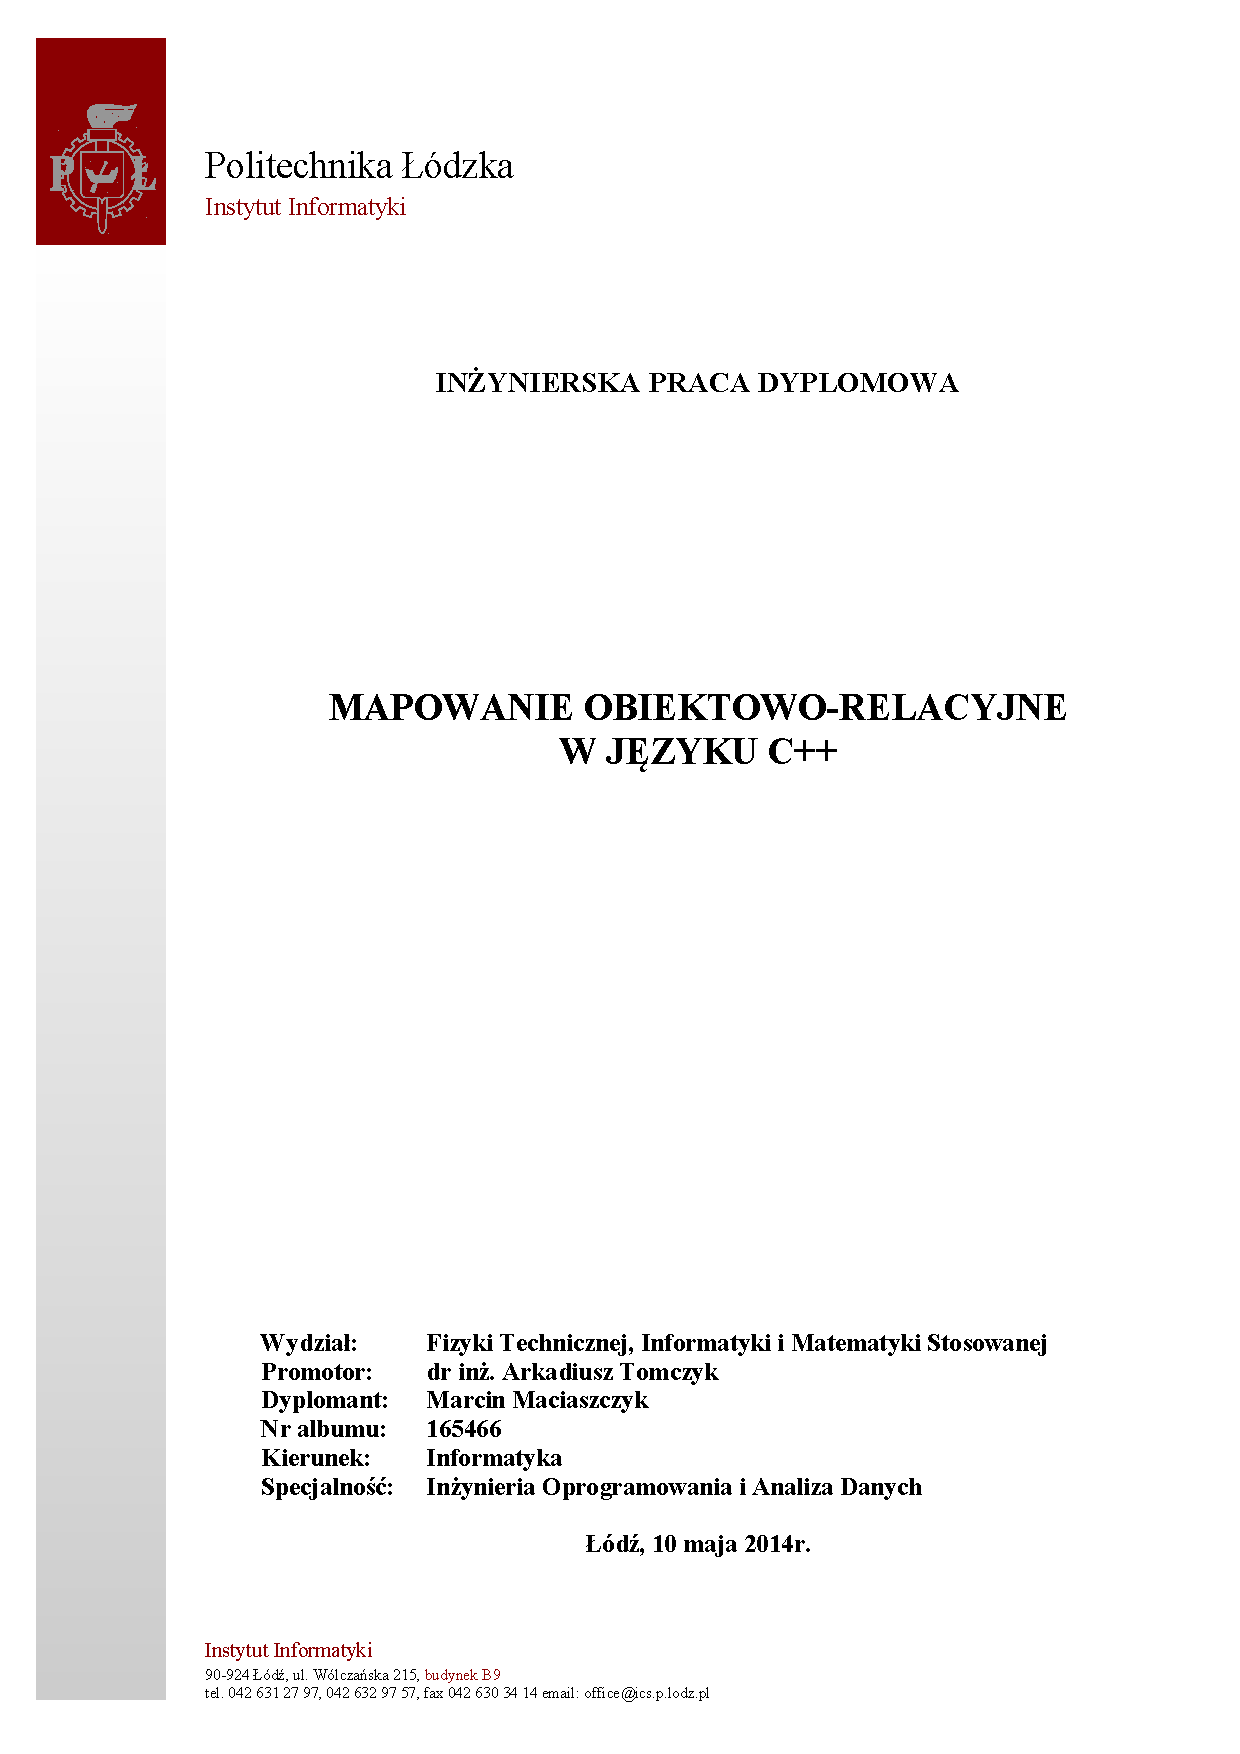
\includepdf[pages={1}]{resources/title_page.pdf}

\tableofcontents

\chapter{Wstęp} \label{wstep}

\section{Uzasadnienie wyboru tematu}

Wraz z upływem czasu postęp technologiczny ma wpływ na życia co raz szerszej rzeszy ludzi na całym świecie. Niezliczone ilości urządzeń zagościły na stałe w domach i mało kto wyobraża sobie bez nich swoje życie. Zaczynając od artykułów gospodarstwa domowego, a kończąc na elektronice użytkowej do której zaliczają się komputery, telewizory czy też smartfony\footnote{~Przenośne urządzenia łączące w sobie zalety telefonów komórkowych oraz przenośnych komputerów (z ang. smartphone).}. Wszystkie te urządzenia mają na celu ułatwianie życia swoim użytkownikom.

W parze z licznymi zaletami urządzeń elektronicznych idą jednak pewne wady. Jedną z istotniejszych jest wpływ czasu spędzanego przed różnego rodzaju wyświetlaczami na zdrowie. Badania przeprowadzone na bazie danych Nielsen Audience Measurement pokazują, że przeciętny Polak spędza dziennie średnio 4,5 godziny przed ekranem telewizora\footnote{~Badania zostały przeprowadzone z uwzględnienem osób powyżej 4 roku życia w okresie od stycznia do czerwca 2015 roku \cite{czasprzedtv}.}. Nie oznacza to jednak, że przez cały ten czas ogląda on telewizję. Oglądanie filmów z dysku komputera, za pomocą serwisów VOD\footnote{~Wideo na życzenie (z ang. video on demand).} czy granie na konsoli także są wliczone w ten czas. Gdyby jednak dodać do tego czas spędzony przed ekranem smartfona czy też komputera wynik byłby zapewne dwukrotnie większy.

% TODO wsparcie co najmniej dwoma żródłami i cos o ogladaniu w ciemnosci
Pogorszenie wzroku czy też wysychanie gałki ocznej są wymieniane jako naj\-częstsze skutki zbyt dużej ilości czasu spędzanego przed ekranem. Poza próbą jego ograniczenia, jedną z częstszych porad jest próba zmniejszenia kontrastu pomiędzy ekranem a jego otoczeniem.

Do celów niniejszej pracy należy złożenie i oprogramowanie systemu oświetlenia, który ma rozszerzać obraz widziany na ekranie na jego otoczenie. Poza zmniejszeniem kontrastu, a więc aspektem zdrowotnym, system ma także na celu zwiększyć wrażenia wizualne dostarczane przez oglądany obraz.

% TODO krótkie wyjaśnienie podstawowych pojęć i diagram/zdjęcia
System oświetlenia składa się z taśmy diod elektroluminescencyjnych\footnote{~LED (z ang. light-emitting diode).} pod\-łączonych do mikrokontrolera Arduino Uno, który z kolei ma współpracować z komputerem z zainstalowanym systemem operacyjnym MacOS. Oprogramowanie mikrokontrolera, którego zadaniem jest sterowanie diodami zostało przygotowane w języku Arduino, natomiast aplikacja kontrolująca cały system przeznaczona na komputer z systemem MacOS zostałą napisana w języku Swift. Wybór języków jest ściśle związany z koniecznością uzyskania jak najlepszej wydajności oraz użyciem najnowszych technologii.

Podobne systemy oświetlenia dostępne są już od pewnego czasu na rynku, jednak to właśnie nowoczesne technologie, prostota wykonania i niskie koszta powinny uczynić z Ligtning, bo taką nazwę otrzymał projekt, pełnowartościowego konkurenta.

\section{Problematyka i zakres pracy}

% TODO problematyka i zakres pracy

\section{Cele pracy}

% TODO cele pracy

\section{Metoda badawcza}

% metoda badawcza

\section{Przegląd literatury w dziedzinie}

% przeglad literatury

\section{Układ pracy}

% uklad pracy

\chapter[Zagadnienia teoretyczne]{Zagadnienia teoretyczne}
\label{teoria}

% TODO teoria

\chapter[Analiza istniejących rozwiązań]{Analiza istniejących rozwiązań}
\label{analiza}

\section{Kryteria analizy}

% TODO kryteria analizy

\section{Porównanie istniejących rozwiązań}

% TODO porownanie

\chapter{System oświetlenia Lightning}
\label{lightning}

% TODO projekt

\section{Moduły tworzonej aplikacji}

% TODO moduly

\section{Analiza wymagań}

% TODO wymagania

\section{Projekt}

% TODO projekt

\section{Implementacja}

% TODO implementacja

\section{Podręcznik użytkownika}

% TODO faq

\section{Przykładowa aplikacja wykorzystująca Qubica}

% TODO rozszerzenia animacje

\section{Analiza Qubica}

% TODO analiza

\section{Perspektywy rozwoju Qubica} \label{perspektywyqubic}

% TODO perspektywy

\chapter{Podsumowanie} \label{podsumowanie}

\section{Dyskusja wyników}

% TODO wyniki

\section{Perspektywy rozwoju pracy}

% TODO praca

\addcontentsline{toc}{chapter}{Bibliografia} 
\begin{thebibliography}{99}
\bibitem{czasprzedtv} {\tt http://www.wirtualnemedia.pl/artykul/coraz-dluzej-ogladamy-telewizje-najwiecej-czasu-przed-szklanym-ekranem-spedzaja-seniorzy-raport}. Data dostępu -- 15.01.2017.
\end{thebibliography}

\addcontentsline{toc}{chapter}{Spis rysunków} 
\listoffigures

\addcontentsline{toc}{chapter}{Spis tabel} 
\listoftables

\addcontentsline{toc}{chapter}{Spis listingów} 
\lstlistoflistings

\end{document}